\defChapterTarget[ImplementationIntegrationAndTestPlan]{Implementation, integration and test plan}
    \section{Implementation plan}
    SafeStreets system is composed by different subsystems:
    \begin{itemize}
        \item MobileApp
        \item WebServerApp
        \item AuhtorityUserWebApp
        \item ApplicationServer
    \end{itemize}   
    All SafeStreets subsystems need to be implemented, tested and integrated
    using a bottom-up approach. With a bottom-up strategy it's possible to
    develop lower level components first and then to reuse them in order to
    create higher level elements. Bottom-up approach also allows better testing
    of all the different components. It's important to show a visible
    application feature during all the steps of the development.\\
    There also are some external subsystems: 
    \begin{itemize}
        \item SafeStreets DBMS
        \item Municipality DBMS
        \item Google Maps
        \item Plate Recognizer
        \item Ghiro
    \end{itemize}   
    All the external subsystems, of course, are not implemented and tested
    because are developed by third parties, therefore, can be already considered
    stable and trustworthy.\\
    Follows a list with all the features, their importance for the customer
    (therefore to the SafeStreets initiative itself) and their complexity of
    implementation in order to have a better estimation of the order and the
    time needed to meet the given requirements.
    \begin{table}[]
        \begin{tabular}{|l|l|l|}
            \hline
            \textbf{Feature} & \textbf{Importance for the customer}  &
            \textbf{Implementation difficulty}  \\ \hline
            SignUp and SignIn & Low  & Low  \\ \hline
            Signal a violation & High  & High  \\ \hline
            Manage previous reports & Medium  & Medium  \\ \hline
            Visualize unsafe areas & High & High  \\ \hline
            Manage Account Settings & High & Low  \\ \hline
            Violation Checking & High & High  \\ \hline
            Visualize Statistics & High & High  \\ \hline
        \end{tabular}
    \end{table}
    
    \newpage
    \section{Integration and testing}
    \subsection{Entry criteria}
    In order to start the integration testing process and to produce meaningful
    results, there are a number of conditions on the progress of the development
    of the project that have to be met. As a matter of fact the integration
    process should start only when the estimated percentage of completion of
    every component with respect to its functionalities is:
    \begin{table}[H]
        \begin{tabular}{|l|l|l|}
            \hline
            \textbf{Feature Of Component} & \textbf{Implementation percentage} &
            \textbf{Comments}\\ \hline
            Accountmanager & 90-95 & \begin{minipage}[t]{0.4\textwidth}The
                functionality of 'Manage Account Settings' is important for the
                user but we can see it as an extra accessory that does not
                affect the other features of the system, and for this reason the
                corresponding component 'AccountManager' can be implemented and
                tested later than the others.\\\end{minipage} \\\hline
                \begin{minipage}[t]{0.4\textwidth}
                    SignUpManager and SignInManager
                \end{minipage} & 80-90 &
                \begin{minipage}[t]{0.4\textwidth}
                    The sign up and sign in features are obviously an entry
                    condition for the right functioning of the system, but they
                    are not core features and they are not very complex, so the
                    testing and implementation of his corresponding components
                    'SignUpManager' and 'SignInManager' can be delayed. \\
                \end{minipage} \\\hline
            \end{tabular}
        
        \end{table}

        \newpage
        \begin{table}[H]
            \begin{tabular}{|l|l|l|}
                \hline
                StatisticsManager & 
                \begin{minipage}[t]{0.4\textwidth}
                    50-60 
                \end{minipage} & 
                \begin{minipage}[t]{0.4\textwidth}
                    The functionality of 'Visualize Statistics' needs to be
                    implemented all the part relating to the reporting and
                    management of them, so its entry percentage can be subsequent to
                    the previous one. The component 'StatisticsManager' can just
                    postpone a bit its testing.\\
                \end{minipage} \\\hline
                \begin{minipage}[t]{0.4\textwidth}
                    UnsafeAreasManager and CrossDataManager 
                \end{minipage} & 50-60 &
                \begin{minipage}[t]{0.4\textwidth}
                    The functionality of 'Visualize Unsafe Areas' has the same
                    role of the previous one, but instead about the Director it's
                    about the Municipal Employee. The components
                    'UnsafeAreasManager' and 'CrossDataManager' can just postpone a
                    bit its testing.\\ 
                \end{minipage} \\\hline
                ViolationsListManager & 20-30 &
                \begin{minipage}[t]{0.4\textwidth}
                    The functionality of 'Manage Previous Reports' it's
                    important both for the users and for the authorities. The
                    authority needs this component to do his job and the user
                    needs this component to track his signalations. So this
                    component needs to be implemented before
                    ViolationsCheckingManager and to be tested as soon as
                    possible.\\
                \end{minipage} \\\hline
                ViolationsCheckingManager & 10-20 &
                \begin{minipage}[t]{0.4\textwidth}
                    The functionality of
                    'Violation Checking' is very important and affect many other
                    features, so it's crucial to implement and test it. The
                    component 'ViolationCheckingManager' it's hard to implement and
                    it needs to be tested as soon as it is ready.\\
                \end{minipage}
                \\\hline
            \end{tabular}
        
        \end{table}

        \newpage
        \begin{table}[H]
            \begin{tabular}{|l|l|l|}
                \hline
                SignalViolationManager & 
                \begin{minipage}[t]{0.4\textwidth}
                    10-15 
                \end{minipage} &
                \begin{minipage}[t]{0.4\textwidth}
                    Signal a violation is the core functionality of the system
                    and without it most other features would make no sense, it
                    requires an implementation and integration with other
                    functionalities as soon as possible. The component
                    'SignalViolationManager' is tested as soon as it is ready.\\
                \end{minipage} \\\hline
        \end{tabular}
        
    \end{table}
        \subsection{Integration testing strategy}
        It is stated, throughout the document, that the integration strategy for
        the SafeStreets software is a bottom-up strategy. Here follows a brief
        description of what this strategy is.

        A \emph{Bottom Up approach} is testing strategy that allows it to be as
        user friendly as it can possibly be and provides a high deployment
        coverage, especially in early phases of the development. The whole
        software is broken into small submodules that can be indipendently
        developed and then, after have been correctly tested, can be linked
        between each other in order to finalise the software requested. By doing
        so, the main faulty interactions are easily exposed and can promptly be
        fixed. Furthermore, by separating the final product in smaller modules,
        the reusability of said modules can be augmented and simply the process
        of creation, in both resources and time.

        \subsection{Sequence of component/function integration}

        \subsubsection{Integration of frontend and backend}
            \begin{figure}[H]
                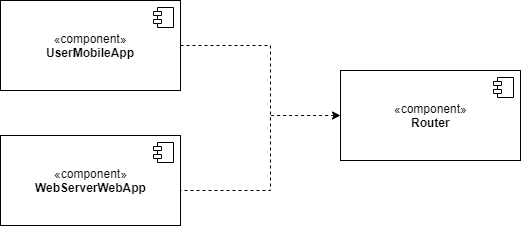
\includegraphics[scale=0.7]{dd/resources/images/Integration-Router.png}
                \caption{Router integration}        
            \end{figure}
            \begin{figure}[H]
                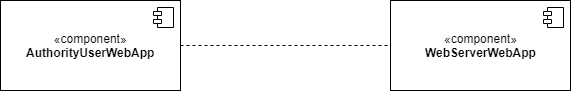
\includegraphics[scale=0.65]{dd/resources/images/Integration-Web.png}
                \caption{AuthorityUserWebApp-WebServerWebApp integration}        
            \end{figure}

        \subsubsection{External services integration}    
            \begin{figure}[H]
                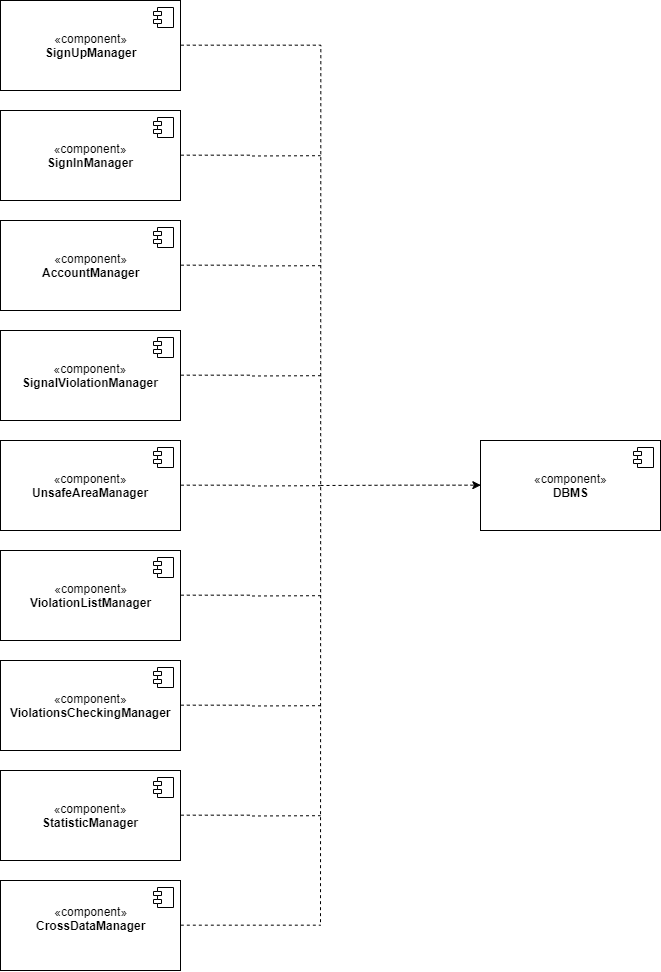
\includegraphics[scale=0.5]{dd/resources/images/Integration-DBMS.png}
                \caption{DBMS integration}        
            \end{figure}
            \begin{figure}[H]
                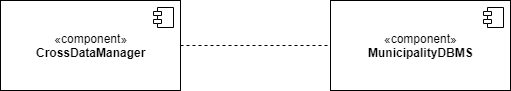
\includegraphics[scale=0.7]{dd/resources/images/Integration-MunicipalityDBMS.png}
                \caption{MunicipalityDBMS integration}        
            \end{figure}
            \begin{figure}[H]
                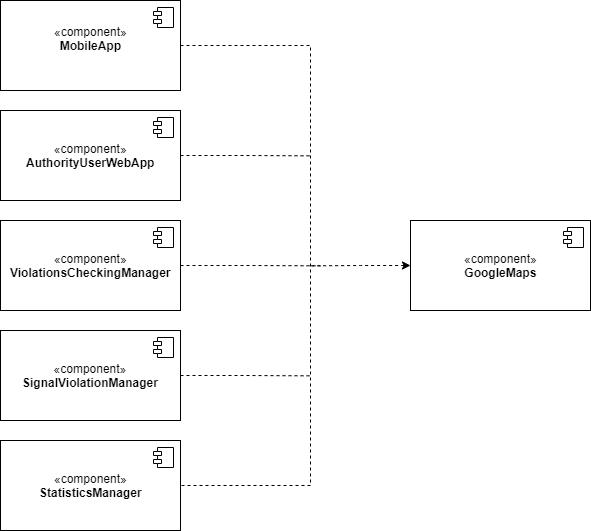
\includegraphics[scale=0.7]{dd/resources/images/Integration-GoogleMaps.png}
                \caption{Google Maps integration}        
            \end{figure}
            \begin{figure}[H]
                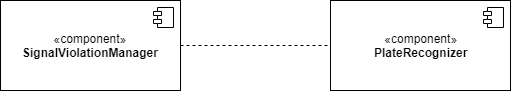
\includegraphics[scale=0.7]{dd/resources/images/Integration-PlateRecognizer.png}
                \caption{Plate Recognizer integration}        
            \end{figure}

        \subsubsection{External services integration}    
            \begin{figure}[H]
                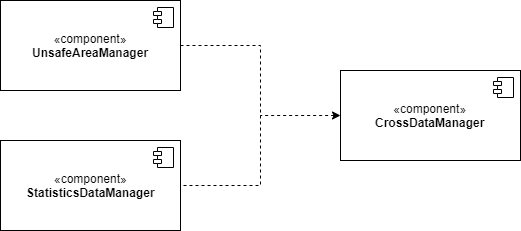
\includegraphics[scale=0.7]{dd/resources/images/Integration-CrossDataManager.png}
                \caption{CrossDataManager integration}        
            \end{figure}